




%----------------------------------------------------------------------
\section{Solution Framework}
%----------------------------------------------------------------------

\begin {figure}[H]
\centering
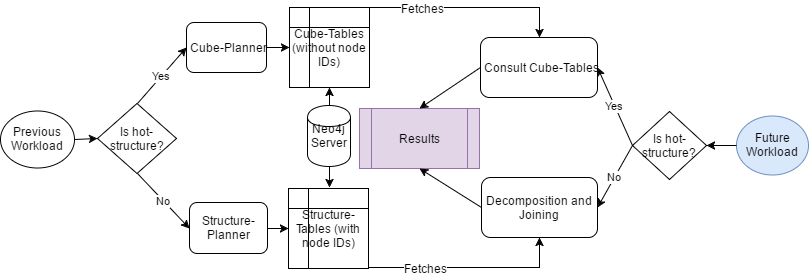
\includegraphics[scale=0.6]{pic/41.png}
\caption{Solution framework.}
\end{figure}

Our solution framework contains two major parts:

Partial Materialization part: Cube-Planner and Structure-Planner select cuboids and substructures to precompute.

Decomposition part: Scan over cuboids or join using substructures to produce results. 

We will discuss Partial Materialization part in Section 4.2 and Decomposition part in Section 4.3.

%----------------------------------------------------------------------
\section{Partial Materialization}
%----------------------------------------------------------------------


In 3.1.2, we have discussed about the trade-off between cuboid and substructures. We know that benefit of a cuboid rely on future queries of exactly same structure. Therefore it is wize that we materizalize cuboids on a structure only when we are fully confident that the structure is of high interest for the client. Otherwize, we may risk wasting space only to materialize cuboids that are rarely "hit" by future queries. On the other hand, substructures are less picky in terms of exact match of future query structures. Therefore we make our partial materialization policy as follows: 

For queries of structure frequency over a threshold, consider these queries have "hot structure" and pass them to CubePlanner for cuboid selection. 

For other queries with "less hot structure", pass them to StructurePlanner for substructure selection. 

\begin{algorithm}[H]
	\caption{PartialMaterialization}
	\LinesNumbered
	\textbf{System setting:} threshold: frequency threshold for hot structures\\ 
	\KwIn{Q: a set of previous queries\\}
	\KwOut{C: a set of materialized cuboids\\ S: a set of materialized substructures}
	
	$CInput \gets \emptyset$ \;
	$SInput \gets \emptyset$ \;
	\ForEach{q \in Q}{
		\eIf{structureFreq(Q, q) $>$ threshold}{
			$CInput \gets CInput \cup \{q\} $\;
		}{	
			$SInput \gets SInput \cup \{q\} $\;
		}
	}
	$C:=materialize(CubePlanner(CInput))$ \;
	$S:=materialize(StructurePlanner(SInput))$\;
\end{algorithm}
\clearpage

For instance:

\textbf{Previous Workload:}

Badge-User, User-Post:Badge-Name,Post-Score,Post-PostTypeId=2

User-Comment, Comment-Post: User-UpVotes, Comment-Score, (AVG)Post-Score, Post-PostTypeId=1

User-Post, Post-Vote: User-UpVotes, Vote-VoteTypeId

User-Post, Post-Tag: (AVG)User-CreationDate_Year, Tag-TagName

User-Comment, Comment-Post: User-ActiveMonth, Post-CreationDate_Year=2016

User-Comment, Comment-Post: User-Age, (AVG)Comment-Score, Post-PostTypeId=2

\textbf{Future Workload:}

User-Comment, Comment-Post: User-UpVotes, (AVG)Post-Score, Post-PostTypeId

User-Comment, Comment-Post: User-Age, Post-PostTypeId

User-Post, Post-PostHistory: User-UpVotes, PostHistory-PostHistoryTypeId

Badge-User, User-Post:(AVG)Post-Score,Post-PostTypeId=2



We count previous queries by structure:

\begin{center}
	\begin{tabular}{ | c | c |}  
		\hline
		Structure	&Frequency	\\ \hline 
		\textbf{User-Comment, Comment-Post} 	&\textbf{3} \\ \hline
		User-Post, Post-Tag 	&1 \\ \hline
		User-Post, Post-Vote	&1 \\ \hline
	\end{tabular}
	\end {center}
	
We are confident that \textit{User-Comment, Comment-Post} is a "hot structure". We materialze cuboids over \textit{User-Comment, Comment-Post} using

User-Comment, Comment-Post: User-UpVotes, Comment-Score, (AVG)Post-Score, Post-PostTypeId=1

User-Comment, Comment-Post: User-ActiveMonth, Post-CreationDate_Year=2016

User-Comment, Comment-Post: User-Age, (AVG)Comment-Score, Post-PostTypeId=2

and hopefully these cuboids benefit processing of future queries

User-Comment, Comment-Post: User-UpVotes, (AVG)Post-Score, Post-PostTypeId

User-Comment, Comment-Post: User-Age, Post-PostTypeId

We pass the rest three queries of "less hot structure" 

Badge-User, User-Post:Badge-Name,Post-Score,Post-PostTypeId=2

User-Post, Post-Vote: User-UpVotes, Vote-VoteTypeId

User-Post, Post-Tag: (AVG)User-CreationDate_Year, Tag-TagName

to StructurePlanner. StructurePlanner will discover most useful substructures. For instance StructurePlanner is likely to find

\textit{User-Post }

as a useful substructure and hopefully the materialized substructure can be used in faster joining the result of 

User-Post, Post-PostHistory: User-UpVotes, PostHistory-PostHistoryTypeId

Badge-User, User-Post:(AVG)Post-Score,Post-PostTypeId=2

%----------------------------------------------------------------------
\subsection{Greedy Selection Framework}
%----------------------------------------------------------------------

Cube-Planner and Structure-Planner adopt the same greedy selection framework. We will discuss this greedy selection framework first so that readers could have a high-level idea of our selection policy.

 Our problem is  

given previous queires P, space limit $\sigma$, select cuboids C and substructures S to materialize so that future workload F processing could be mostly benefited. Suppose P and F consist of similar queries.
 
We used greedy algorithms for cuboid and substructure selection. The idea is to always pick next candidate with highest ratio of margin benefit/space. After a candidate is picked, re-evaluate benefit of the rest candidates. Re-evaluation is essential as margin benefit of a candidate may be influenced after materializaion of another candidate.


\begin{algorithm}[H]
	\caption{Greedy Selection}
	\LinesNumbered  
	\textbf{System setting:} $\sigma$: space limit\\ 
	\KwIn{C: a set of candidates of cuboids or substructures in lattice structure\\ P: A set of previous queries}
	\KwOut{Q: a queue of selected candidates to materialize\\ }
	\ForEach{c \in C}{
		c.space := estimateSpace(c) \;
		c.benefit := estimateMarginBenefit(c, P, Q) \;
		c.score := c.benefit/c.space \;
	} 
	
	\For{$Q.totalsize < \sigma$}{
		selected := c in C with highest score \;  
		Q.offer(selected)\;
		repeat 1-5 \;
	}
\end{algorithm}

1-5 estimates space cost, marginal benefit for future workload, and score for each candidate. We call this parse  "score calculation".

6-10 keeps picking up candidates with highest score one by one until space limit is hit. Notice that each time a candidate is selected, 9 refreshes scores for all candidates by repeating 1-5. We call this parse "pick-and-update".   

Cube-Planner and Structure-Planner apply this greedy selection framework with specific implementation of score caculation in 1-5. Future users can plug-in their implementation and design their planners with consideration of their database settings. We will introduce how we implement our Cube-Planner and Structure-Planner for Neo4j in the following sections.
 
%----------------------------------------------------------------------
\subsection{Cuboid Planner}
%----------------------------------------------------------------------  

%----------------------------------------------------------------------
\subsubsection{Single Cube}
%----------------------------------------------------------------------  

Given previous queries of a same structure, we implement  SingleCubePlanner from greedy selection framework to select cuboids. 

\begin{algorithm}[H]
	\caption{SingleCubePlanner}
	\LinesNumbered 
	\textbf{System setting:} n: maximum number of cuboids to precompute\\ 
	\KwIn{P: a set of previous queries with a same structure}
	\KwOut{C: an queue of selected cuboids to precompute\\ }
	$Lattice \leftarrow buildLattice(Q)$\;
	\ForEach{query q \in P}{
		$q.time \leftarrow estimateProcessingTime(q)$ \;
	} 
	\ForEach{cuboid \in Lattice}{
		$cuboid.space \leftarrow estimateSpace(cuboid) $\;
		$cuboid.benefit \leftarrow 0$\;
		\ForEach{query q $\in$ P and q.properties $\subseteq$ cuboid.properties}{
			$cuboid.benefit +=max(0, q.time-estimateScanningTime(cuboid))$\;
		}
		$cuboid.score \leftarrow cuboid.benefit/cuboid.space$ \;
	}
	\For{i=1 \emph{\KwTo} n}{
		nextBestCube $\gets$ cuboid in Lattice with highest score \;
		\If{$nextBestCube.score < 0$}{
			break \;
		}
		C.offer(nextBestCube)\;
		\ForEach{cuboid q $\in$ Q and q.dimension $\subseteq$ nextBestCube.dimension }{
			$q.time \gets min(q.time, estimateScanningTime(nextBestCube)) $\;
		}
		repeat 5-12 \;
	}
	
\end{algorithm}
\clearpage

1 builds a lattice over all conbinations of dimensions of all attributes that appeared in previous queries P, using classic lattice construction algorithms.

2-4 initializes best-so-far processing time for each previous query by its naive database processing time.

5-12 performs "score calculation". For each cuboid, 6 estimates its space. 8-10 iterates over all "roll-up" previous queries adds on marginal benefit if scanning time over the cuboid is smaller than a previous "roll-up" query's best-so-far processing time.

13-23 performs "pick-and-update". 15-17 terminates selection when there is no marginal benefit at all. 19-22 updates best-so-far processing time for previous queries as a result of current round of selection.

Implementation of functions are listed as follows. Notice that users can implement in their own ways based on their database systems. 

Function estimateProcessingTime(query) provides naive estimated time cost of processing a query with a graph database. Implementation of estimateProcessingTime(query) is database specific as physical storage execution plans vary among different databases. Some graph databases like Neo4j provide APIs to see the execution plan and estimated intermediate size. In our implementation we used total size of intermediate results as estimation of time cost.
  
Execution plan of Cypher query:

match (u:User)-[]-(b:Badge)  match (u:User)-[]-(p:Post)  match (p:Post)-[]-(t:Tag)  return  t.TagName, count(*)

\begin {figure}[H]
\centering
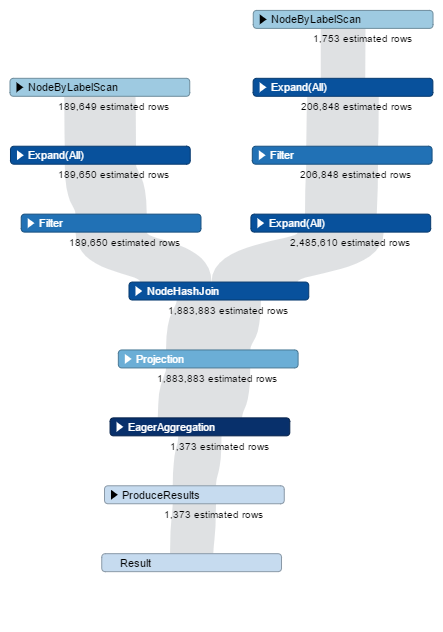
\includegraphics[scale=0.6]{pic/61.png}
\end{figure}

If APIs to see the execution plan and estimated intermediate result sizes are not provided for graph databases, we need to estimate in our own way. There are many studies about joining cost estimation. The key issue is to determine joining order and estimate intermediate result sizes using selectivity. Joining estimation [6] is a good summary of different joining plans and ways of cost estimation. 

Function estimateScanningTime(cuboid) estimates time cost for scanning cuboid result. For cuboid C. We use space cost of cuboid result table for estimation. 

 $spacePerRow:= 
 \displaystyle{\sum_{p\in C.properties}sizeOf(p)}$
 
$SpaceCost(C):= spacePerRow *  numberOfRows(C)$
 
Here sizeOf(property type) refers to standard size of data types. For instance int type in C is 2 byte.

numberOfRows(C) refers to number of rows of C. A rough estimation is product of candinalities of each property.  We added a shrinking effect because some conbinations of property values do not exsist in the final result. 
 
$numberOfRows(C):= \displaystyle{\prod_{p\in C.properties}|p|} * shrinking\_factor^{|C.properties|-1}$

%----------------------------------------------------------------------
\subsubsection{Holistic Cube}
%---------------------------------------------------------------------- 

SingleCubePlanner selects cuboids from one lattice of one structure. However the input to CubePlanner may consist of previous queries of various hot structures. CubePlanner performs cuboid selection in a holistic manner by calling SingleCubePlanner for each hot structure and rank cuboids across different lattices(cubes). 

\begin{algorithm}[H]
	\caption{CubePlanner}
	\LinesNumbered 
	\textbf{System setting:} n: maximum number of cuboids to precompute\\ 
	\KwIn{Q: a set of previous queries not nessesarily with a same structure}
	\KwOut{C: a queue of selected cuboids to precompute\\ }
	Group:= GroupByStructure(Q) \;
	\ForEach{group \in Group}{
		group.candidates := SingleCubePlanner(group);
	} 
	
	\For{i=1 \emph{\KwTo} n}{
		selectedGroup := group in Group with highest group.candidates.top().score \; 
		C.offer(selectedGroup.poll())\;
	}
	
\end{algorithm}
\clearpage

1 partitions Q by structure. Each partition consists of previous queries of a same structure, which could be passed to SingleCubePlanner.

2-4 performs cuboid selection in each partition(cube). An ordered queue of candidates is generated for each partition(cube).

5-8 iteratively checks top candidate for each partition(cube) and picks out the best candidate among them.   

%----------------------------------------------------------------------
\subsection{Structure Planner}
%----------------------------------------------------------------------

\begin{algorithm}[H]
	\caption{StructurePlanner}
	\LinesNumbered 
	\textbf{System setting:} n: maximum number of substructures to precompute\\ 
	\KwIn{Q: a set of previous queries}
	\KwOut{S: an queue of selected substructures to precompute\\ }
	$Lattice \leftarrow buildSubstuctureLattice(Q)$\;
	\ForEach{q \in Q}{
		$q.coveredSubstructre:= \emptyset $\;
	} 
	\ForEach{substructure \in Lattice}{
		$substructure.space \leftarrow estimateSpace(substructure) $\;
		$substructure.benefit \leftarrow 0$\;
		\ForEach{q $\in$ Q and q.structure $\subseteq$ substructure.structure}{
			$cuboid.benefit +=max(0, benefit(q, substructure, q.coveredSubstructre))$\;
		}
		$substructure.score \leftarrow substructure.benefit/substructure.space$ \;
	}
	\For{i=1 \emph{\KwTo} n}{
		nextBestSubstructre $\gets$ substructure in Lattice with highest substructure.score \;
		\If{$nextBestSubstructre.score < 0$}{
			break \;
		}
		S.offer(nextBestSubstructre)\;
		\ForEach{q $\in$ Q and q.structure $\subseteq$ nextBestSubstructre.structure }{
			$q.coveredSubstructre \gets q.coveredSubstructre \cup \{nextBestSubstructre \} $\;
		}
		repeat 5-12 \;
	}
	
\end{algorithm}
\clearpage

1 builds a lattice over all substructures are covered in previous queries P, using classic lattice construction algorithms.

\begin {figure}[H]
\centering
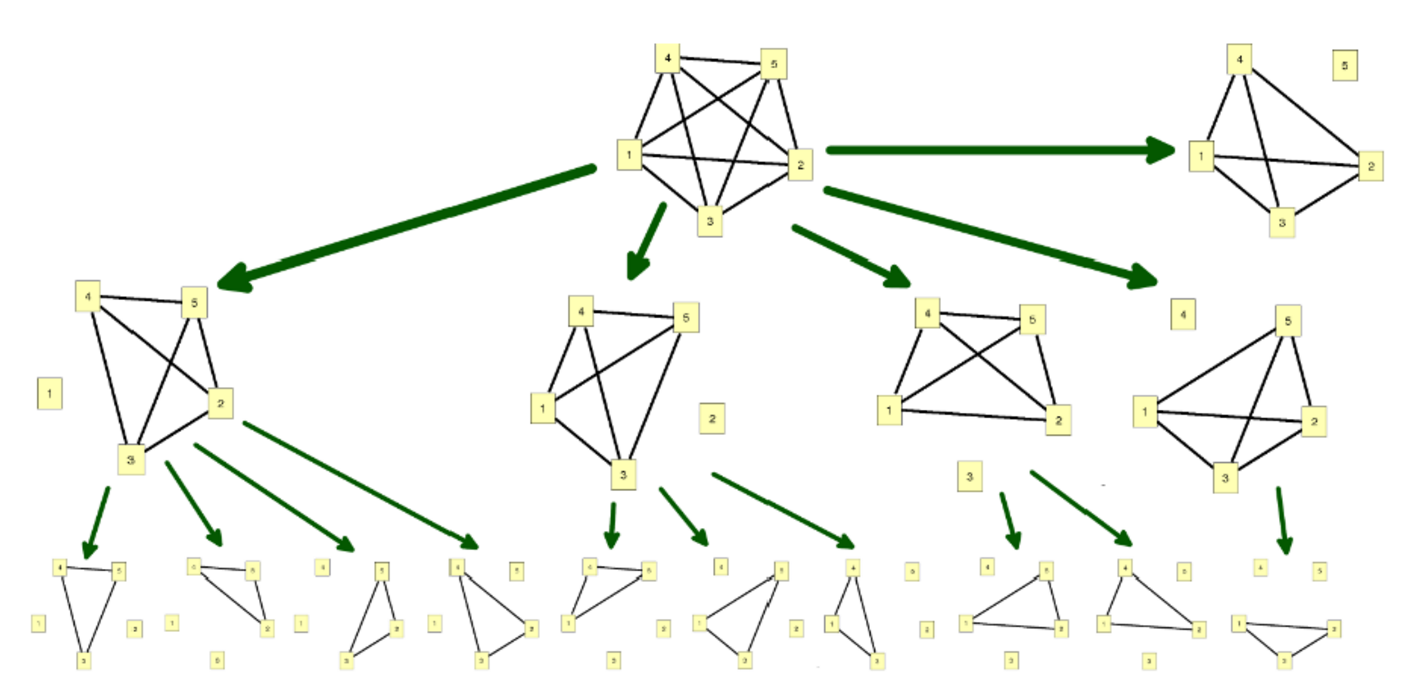
\includegraphics[scale=0.2]{pic/42.png}
\caption{Substructure lattice.}
\end{figure}


2-4 initializes covered substructure for each previous query as empty.

5-12 performs "score calculation". For each substructure, 6 estimates its space. 8-10 iterates over all "favored" previous queries and adds on marginal benefit if any. Here marginal benefit refers to the time saved by adding current substructure to the selected covered substructures.   

13-23 performs "pick-and-update". 15-17 terminates selection when there is no marginal benefit at all. 19-22 updates covered substructures for previous queries as a result of current round of selection.

Implementation of functions are listed as follows. Notice that users can implement in their own ways based on their database systems. 



 Function benefit(q, substructure, q.coveredSubstructre) evaluates marginal benefit of substructure to query q provided that q.coveredSubstructre has been materialized. Such estimation is tricky as using materialized substructure may change original joining plan. Thus estimation on intermediate result sizes is nessasary.  We used 
 
 $estimateProcessingTime(q.coveredSubstructre \cup substructure) - estimateProcessingTime(q.coveredSubstructre)$
 
 for estimation. As we think that this roughly indicates improvement of adding $substructure$ in terms of  reduction of hard-disk access and joining operations. 
 


%----------------------------------------------------------------------
\subsection{ID and Property Selection}
%----------------------------------------------------------------------

Given a substructure picked by Structure Planner, we need to decide on which IDs and attributes to be stored. Taking all IDs and attributes into account will assure that the structure could be used in any future query which covers it but will on the other hand increase space cost. We are faced with a tradeoff between space and potential usage spectrum.

\textbf{IDs:}
\begin{itemize}
	\item Include IDs of all nodes and edges. This would allow “overlap joining” of substructures but increases space cost.
	\item Include IDs of only outer nodes. This saves space cost but does not allow “overlap joining” of substructures.
	
\end{itemize}


Our suggestion is to consider the “expansion” effect of inner nodes' IDs towards space cost. In our implementation, inner nodes' IDs are kept. However if adding inner nodes' IDs overwhelmingly increase resulting table length, then we may choose to ignore inner nodes' IDs as the overhead on space cost is too much. 

\textbf{Attributes:}

\begin{itemize}
	\item Include all attributes.
	\item Include only attributes that appears in previous workloads.
	
\end{itemize}
 
Our suggestion is to consider the portion of attributes that appeared over all attributes in the data schema. For instance, in our experiment only a small portion of attributes were aggregated, therefore it is more of a waste of space to keep all attributes in the data schema.


%----------------------------------------------------------------------
\section{Query Processing}
%----------------------------------------------------------------------
Problem:

Given materialization of cuboids C and substructures S how to process future queries F as fast as possible using C and S? 

Generally speaking, aggreation on cuboid is faster than joining substructures. When future query q arrives, we first consult materializion of cuboids. If any cuboids get "hit" by q, then we select the cuboid of minimum space to aggregate the result of q. If no cuboid gets "hit" by q, then we decompose q and use substructures to compose the result of q. 

\begin{algorithm}[H]
	\caption{FutureQueryProcessing}
	\LinesNumbered
	\textbf{System:} C: a set of materialized cuboids\\ S: a set of materialized substructures\\ 
	\KwIn{q: a future query\\}
	\KwOut{r: result of q}
	
	$minspace:= \infty $\;
	mincuboid := NULL \;
	\ForEach{$cuboid \in C$}{
		\If{cuboid.structure = q.structure and q.dimension \subseteq cuboid.dimension}{
			\If{cuboid.space<minspace}{
				minspace := cuboid.space \;
				mincuboid := cuboid \;
			}
		}

	\eIf{mincuboid \not= NULL}{
		r := aggregate(mincuboid, q);
	}{
		r:=Decompose\_Join(q);
	}
	}
\end{algorithm}
\clearpage

4-9 looks up materialized cuboids and find if there is any "hit". If there are multiple "hits" use the cuboid with the smallest scanning cost.






%----------------------------------------------------------------------
\subsection{Substructure Selection}
%----------------------------------------------------------------------

Given a future query q and materialized substructures S, which substructures shall we select to compose q? Obviously selected substructure s must hold s.structure \subseteq q.structure.
 
However, candidate substructures in S may overlap:

For instance suppose

q.structure : Badge-User, User-Post, Post-Tag

And S consists of substructures 

(1)Badge-User

(2)Badge-User, User-Post 

(3)User-Post, Post-Tag

(4)Post-Tag

(5)User-Post

Then we may have at least three ways of substructure selection.

(1) and (2)

(3) and (4)

(1), (4) and (5)

We propose a greedy algorithm for substructure selection. The idea is to always pick up next substructure with highest heuristic score. Example heuristics are #edges of sub-structure, Score when selected by Structure-Planner, #tuples in the table etc. 

\begin{algorithm}[H]
	\caption{SelectSubstrucre}
	\LinesNumbered
	\textbf{System:} S: a collection of materialized substructures\\ heuristic: heuristic for ordering S\\
	\KwIn{q: a future query\\}
	\KwOut{V : selected views for future joining\\ uncoveredStruc: structure not covered by selected views\\uncoveredProp: properties not covered by selected views\\}
	uncoveredStruc := q.structure \;
	uncoveredProp:= q.properties \; 
	$coveredStruc:= \emptyset$ \;
	$V:=\emptyset $\;
	\ForEach{$s \in S$ ordered by heuristic}{
		\If{s $\subseteq$ uncoveredStruc and s $\not\subseteq$ coveredStruc}{
			$V := V \cup \{s\}$\;
			$coverdStruc := coveredStruc \cup s.structure$ \;
			uncoveredStruc := uncoveredStruc - s.structure \;
			uncoveredProp := uncoveredProp -s.properties\;
		}
	}
\end{algorithm}
\clearpage

5 iterates substructures by user-defined heuristics. 

6 assures that a candidate substructure that is totally covered by selected substructures will be dequalified as major effect of the candidate is already occupied. 

%----------------------------------------------------------------------
\subsection{Query Decomposition}
%----------------------------------------------------------------------

Given future query q, we use SelectSubstrucre to select materializaion V. For the q's remaining structure and properties that V does not cover, we have to retrieve them from database server. Finally we join and aggregate all materials together to produce results.

%----------------------------------------------------------------------
\subsubsection{Decompose\_Join}
%----------------------------------------------------------------------

\begin{algorithm}[H]
	\caption{Decompose\_Join}
	\LinesNumbered
	\textbf{System:} S: a collection of materialized substructures\\ heuristic: heuristic for ordering S\\
	\KwIn{q: a future query\\}
	\KwOut{r: result of q}
	$\Sigma \gets \emptyset $\;
	$V, uncoveredStruc, uncoveredProp \gets SelectSubstrucre(q) $\;
	$\Sigma \gets \Sigma \cup V $\;
	Splits:=split(uncoveredStruc, uncoveredProp)\;
	\ForEach{s: Splits}{
		$\Sigma \gets \Sigma \cup \{materialize(s)\} $\;
	}
	r := join(\Sigma)\;
\end{algorithm}

1 initializes $\Sigma$, which stores all materials that are needed.

2 selects substructures using SelectSubstructure algorithm. $uncoveredStruc$, $uncoveredProp$ are structures and properties not covered. They need to be retrieved from database servers.

4, splits uncoveredStruc and uncoveredProp into connected components. We will retrieve each connected component from database server. Nocice that uncoveredStruc may not be exactly one connected component.

8 joins and aggregates all materials together to produce results. 

Function split(uncoveredStruc, uncoveredProp) is implemented by classic connected components decomposation algorithms.

Function join($\Sigma$) can be implemented with  different table-joining strategies. In our implementation we keep joining two tables which have common colmn(s) and with minimum sum of table sizes. That is, we always select small tables to join.  

%----------------------------------------------------------------------
\subsubsection{$Decompose\_Join_{informative}$}
%----------------------------------------------------------------------
Alternatively, we may adopt the idea of Semi-Join. We first join V. The process of joining has a "filtering" effect. When we retrieve uncovered components from database server, we inform database server with the screened out IDs information. We name this approach "informative materialization". "Informative materialization" may accerlate retrieval from backend databases in two aspects:

First, since screened out IDs are provided, database backend only need to search within screened out IDs. This will reduce database processing time.

Second, size of retrieval results can be deducted. Thus time of transporting results will be reduced. 


\begin{algorithm}[H]
	\caption{$Decompose\_Join_{informative}$}
	\LinesNumbered
	\textbf{System:} S: a collection of materialized substructures\\ heuristic: heuristic for ordering S\\
	\KwIn{q: a future query\\}
	\KwOut{r: result of q}
	$\Sigma \gets \emptyset $\;
	$V, uncoveredStruc, uncoveredProp \gets SelectSubstrucre(q) $\;
	V:=join(V)\;
	$\Sigma \gets \Sigma \cup V $\;
	Splits:=split(uncoveredStruc, uncoveredProp)\;
	\ForEach{s: Splits}{
		$\Sigma \gets \Sigma \cup \{materialize_{informative}(s, V)\} $\;
	}
	r := join(\Sigma)\;
\end{algorithm}
\clearpage

Decompose\_Join perform joining after everything is ready. Unlike Decompose\_Join, we first join V in 3 before retrieval from databases(7). Note that substructures in V may reside in multiple connected components. Thus join(V) may result to multiple Intermediate tables.

In 7, $materialize_{informative}$ fetches results from databases by passing candidate ID information "screened-out" from 3. For instance, Neo4j supports such operations of passing a list of IDs as arguments.

------------------
\subsubsection{$Decompose\_Join_{decisive}$}
%----------------------------------------------------------------------
However "Informative materialization" creates an overhead of transport of screened out IDs. We propose a decisive way to evaluate the trade-off between overhead and benefits of "Informative materialization" and choose between "Informative materialization" and "normal materializaiton".

\begin{algorithm}[H]
	\caption{$Decompose\_Join_{decisive}$}
	\LinesNumbered
	\textbf{System:} S: a collection of materialized substructures\\ heuristic: heuristic for ordering S\\
	\KwIn{q: a future query\\}
	\KwOut{r: result of q}
	$\Sigma \gets \emptyset $\;
	$V, uncoveredStruc, uncoveredProp \gets SelectSubstrucre(q) $\;
	V:=join(V)\;
	$\Sigma \gets \Sigma \cup V $\;
	Splits:=split(uncoveredStruc, uncoveredProp)\;
	\ForEach{s: Splits}{
		\eIf{decide\_informative(s,V)}{
			$\Sigma \gets \Sigma \cup \{materialize_{informative}(s, V)\} $\;
		}{
			$\Sigma \gets \Sigma \cup \{materialize(s)\} $\;
		}
	}
	r := join(\Sigma)\;
\end{algorithm}
\clearpage

In 7, Function decide\_informative(s,V) determines between $materialize_{informative}$ or not. In our implementation we caculates ratio of estimated reducted result size by $materialize_{informative}$, divided by size of input overhead. We make decision by comparing the ratio with a threshold.
